\section{Conformer-CTC: Non-autoregressive ASR}

\begin{frame}{}
    \LARGE \textbf{Conformer-CTC: Non-autoregressive ASR}
\end{frame}

\begin{frame}{Conformer-CTC Overview}
    \begin{columns}
        \begin{column}{0.6\textwidth}
            \begin{itemize}
                \setlength{\itemsep}{1.5em}
                \item \textbf{Conformer:} Combines convolutional and transformer layers.
                \item \textbf{CTC Loss:} Connectionist Temporal Classification for sequence alignment.
                \item \textbf{Non-autoregressive:} Processes entire input sequence in parallel.
            \end{itemize}
        \end{column}
        \begin{column}{0.5\textwidth}
            \begin{center}
                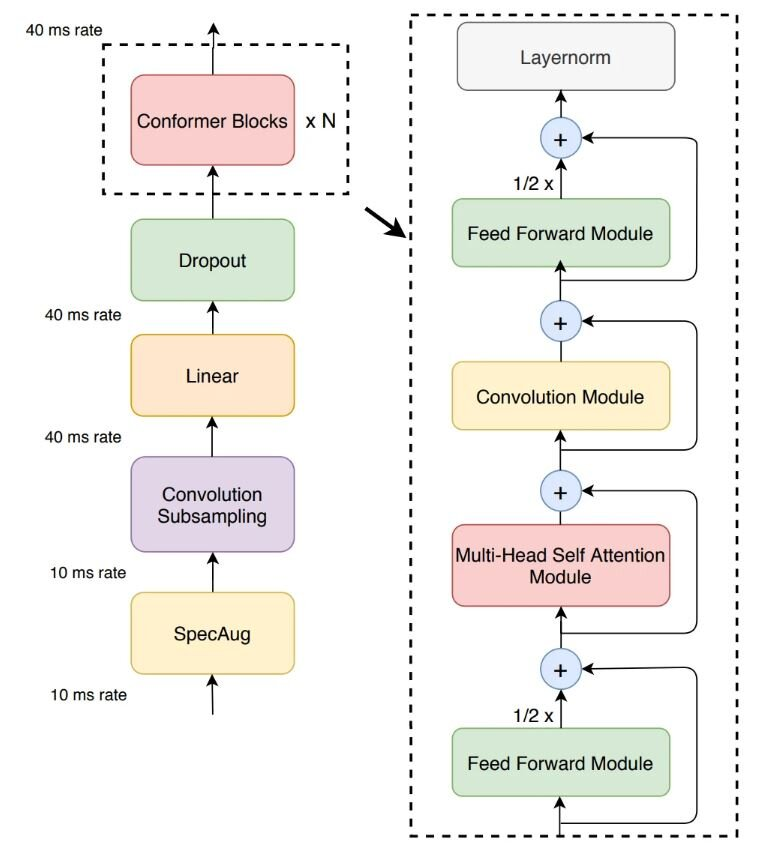
\includegraphics[width=\textwidth,height=0.9\textheight,keepaspectratio]{images/audio-nlp/conformer-ctc.png}
            \end{center}
        \end{column}
    \end{columns}
\end{frame}

\begin{frame}{CTC vs Transducer Models}
    \begin{columns}
        \begin{column}{0.6\textwidth}
            \begin{itemize}
                \setlength{\itemsep}{1.5em}
                \item \textbf{CTC (Connectionist Temporal Classification):}
                \begin{itemize}
                    \item Aligns input and output sequences without explicit segmentation.
                    \item Suitable for non-autoregressive models.
                    \item Decodes output in parallel.
                    \item Simpler and faster inference.
                \end{itemize}
                \item \textbf{Transducer Models:}
                \begin{itemize}
                    \item Jointly model alignment and output prediction.
                    \item Typically autoregressive.
                    \item Better for streaming and online decoding.
                    \item More complex, higher accuracy in some cases.
                \end{itemize}
            \end{itemize}
        \end{column}
        \begin{column}{0.5\textwidth}
            \begin{figure}
                \centering
                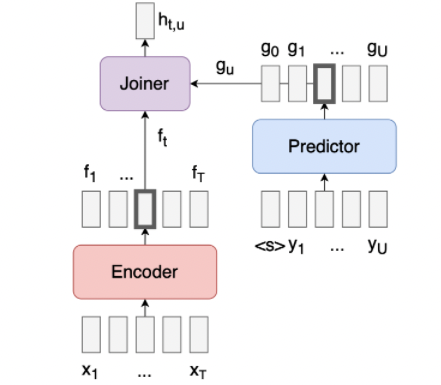
\includegraphics[width=\textwidth]{images/audio-nlp/transducer.png}
                \caption*{An Overview of Transducer Models for ASR.}
            \end{figure}
        \end{column}
    \end{columns}
\end{frame}

\begin{frame}{Conformer-CTC: NVIDIA Implementations}
    \begin{columns}
        \begin{column}{0.5\textwidth}
            \begin{itemize}
                \setlength{\itemsep}{1.5em}
                \item \textbf{NVIDIA Riva:} Production-grade ASR toolkit.
                \item \textbf{Parakeet:} Efficient Conformer-CTC variant.
                \item \textbf{Citrinet:} Convolutional CTC model for fast inference.
                \item Optimized for GPU acceleration.
                \item Supports real-time and batch processing.
            \end{itemize}
        \end{column}
        \begin{column}{0.6\textwidth}
            \begin{center}
                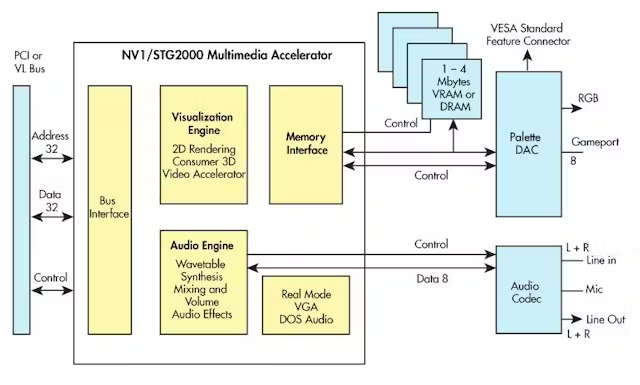
\includegraphics[width=0.9\textwidth]{images/audio-nlp/nvidia-riva.png}
            \end{center}
            \tiny Source: NVIDIA Docs, arXiv
        \end{column}
    \end{columns}
\end{frame}

\begin{frame}{Tech Science: Conformer-CTC Advances}
    \begin{itemize}
        \setlength{\itemsep}{1.5em}
        \item \textbf{Conformer:} Integrates self-attention and convolution.
        \item \textbf{CTC Loss:} Enables parallel decoding.
        \item \textbf{Variants:} Parakeet, Citrinet, and others.
        \item \textbf{Performance:} State-of-the-art on LibriSpeech, CommonVoice.
        \item \textbf{References:}
        \begin{itemize}
            \item \href{https://arxiv.org/abs/2005.08100}{Conformer Paper (arXiv)}
            \item \href{https://docs.nvidia.com/deeplearning/riva/user-guide/docs/reference/models/asr.html}{NVIDIA Riva Docs}
        \end{itemize}
    \end{itemize}
\end{frame}

\begin{frame}{Streaming ASR with SpeechBrain}
    \begin{itemize}
        \item \textbf{SpeechBrain:} Open-source toolkit for speech processing.
        \item Supports streaming ASR with Conformer-CTC.
        \item Easy integration and deployment.
    \end{itemize}
    \begin{center}
        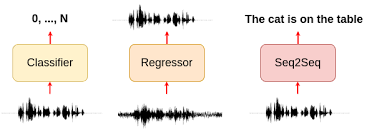
\includegraphics[width=\textwidth]{images/audio-nlp/speechbrain-streaming.png}
    \end{center}
\end{frame}

\begin{frame}{Summary: Non-autoregressive ASR}
    \begin{itemize}
        \setlength{\itemsep}{1.5em}
        \item Conformer-CTC enables fast, parallel ASR.
        \item CTC models are simpler and efficient.
        \item NVIDIA and SpeechBrain provide robust implementations.
        \item Streaming support is available for real-time applications.
    \end{itemize}
\end{frame}